\chapter{Unit Tests}

Bei der Erstellung der Tests wurde stets versucht auf die ATRIP-Regeln zu beachten. Die einzelnen Punkte sind im folgenden genauer aufgeführt.

\paragraph{Automatic}
Damit die Tests eigenständig ablaufen und ihre Ergebnisse selbst überprüfen, wird xUnit verwendet. D.h. die Tests werden als \glqq Fact\grqq{} annotiert und können dann automatisch ausgeführt werden. Es sind keine Benutzereingaben bei den Tests erforderlich und sie liefern immer das Ergebnis \glqq bestanden\grqq{} oder \glqq nicht bestanden\grqq{}.

\paragraph{Thorough}
Der Fokus wurde darauf gelegt das Wichtigste zu testen. Allerdings sind auch manche weniger relevanten Klassen abgedeckt, welche sich einfach Testen lassen und die Test Erstellung daher schnell ging. Ein Beispiel dafür ist der \href{https://github.com/EinToni/Wortfinder/blob/main/Wortfinder/GameScore.cs}{\textit{GameScore}}, welcher die Punkte des aktuellen Spiels zählt, somit nicht Missions-kritisch ist, aber dennoch abgedeckt wurde. Es wurde allerdings auch nicht jede wichtige Funktionalität getestet. Beispiele hierfür sind die GUI oder der \href{https://github.com/EinToni/Wortfinder/blob/main/Wortfinder/MainWindowController.cs}{\textit{MainWindowController}}, welcher die Steuerung des Hauptfensters übernimmt und daher sehr wichtig ist, aber nicht vollständig durch Tests abgedeckt ist.
%% Mehrere Szenarien abgedeckt

\paragraph{Repeatable}
Durch die Nutzung von xUnit lassen sich die Tests jederzeit auf Knopfdruck automatisch ausführen. Die Ergebnisse haben bis Dato immer das gleiche Ergebnis geliefert und sollten dies auch weiterhin, da keine direkten Festplattenzugriffe oder Zeitabhängige Funktionen getestet wurden. 

\paragraph{Independent}
Die Tests sind unabhängig voneinander. Außerdem werden sie durch xUnit in einer unbekannten Reihenfolge ausgeführt.

\paragraph{Professional}
Es wurde versucht den Testcode möglichst einfach, leserlich und kurz zu halten. Für das bessere Verständnis wurden meistens erklärende Variablen eingeführt, anstelle die Werte direkt zu verwenden. Allerdings wurde im Nachhinein festgestellt, dass dies nicht immer eingehalten wurde. Vor allem bei sehr kurzen Tests wurde auf extra Variablen verzichtet. In der folgenden Abbildung sieht man links einen einfach verständlichen Test mit extra Variablen und rechts einen Test ohne extra Variablen, welcher dafür aufgrund der Kürze immer noch recht verständlich ist.

\begin{figure}[!htb]
\centering
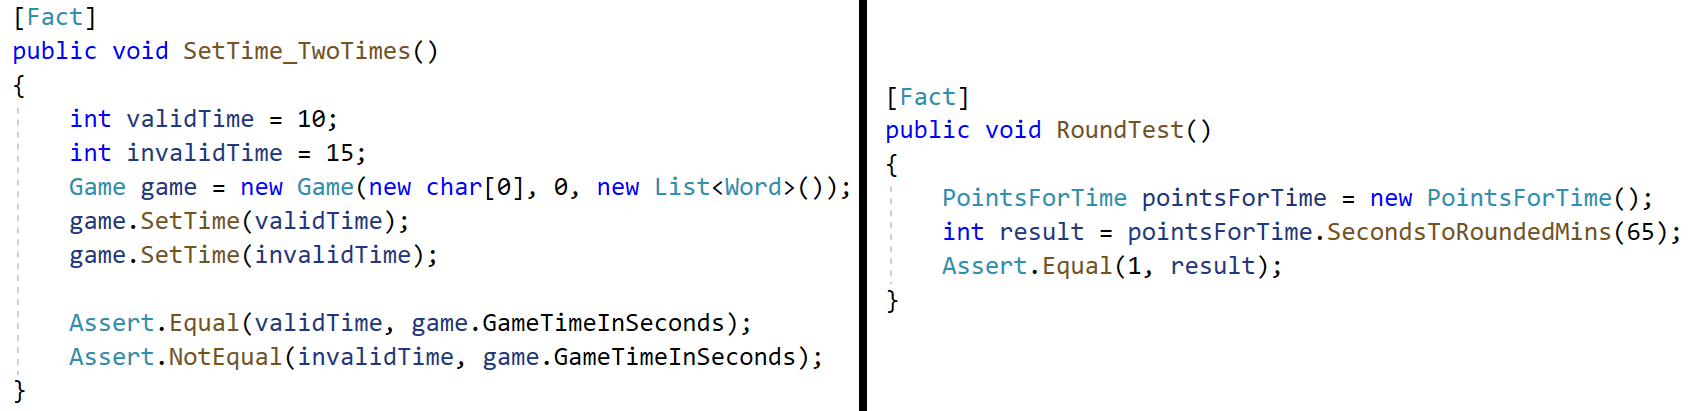
\includegraphics[width=0.95\textwidth]{Bilder/professional_example.PNG}
\caption{\label{Abb:professional_example} Professional Beispiel in ATRIP}
\end{figure}


\paragraph{Struktur}
Die Tests wurden in der AAA-Normalform erstellt. Mock-Objekte wurden mit Moq erstellt. Ein Beispiel für die Normalform sowie die Verwendung von Mocks ist nachfolgend dargestellt. Dabei werden im \glqq Arrange\grqq{} Part 5 Mocks erstellt, da diese im Konstruktor der Klasse benötigt werden und anschließend eine Instanz der Klasse erzeugt. Die Mocks werden nicht weiter konfiguriert, da sie nur für die Dependency Injection im Konstruktor benötigt werden, aber nicht für den eigentlichen Test. Danach folgt der \glqq Act\grqq{}, d.h. die Ausführung in welchem die zu testende Funktion aufgerufen wird. Abschließend folgt der \glqq Assert\grqq{} Teil, in welchem überprüft wird ob das Ergebnis korrekt ist.


\begin{figure}[!htb]
\centering
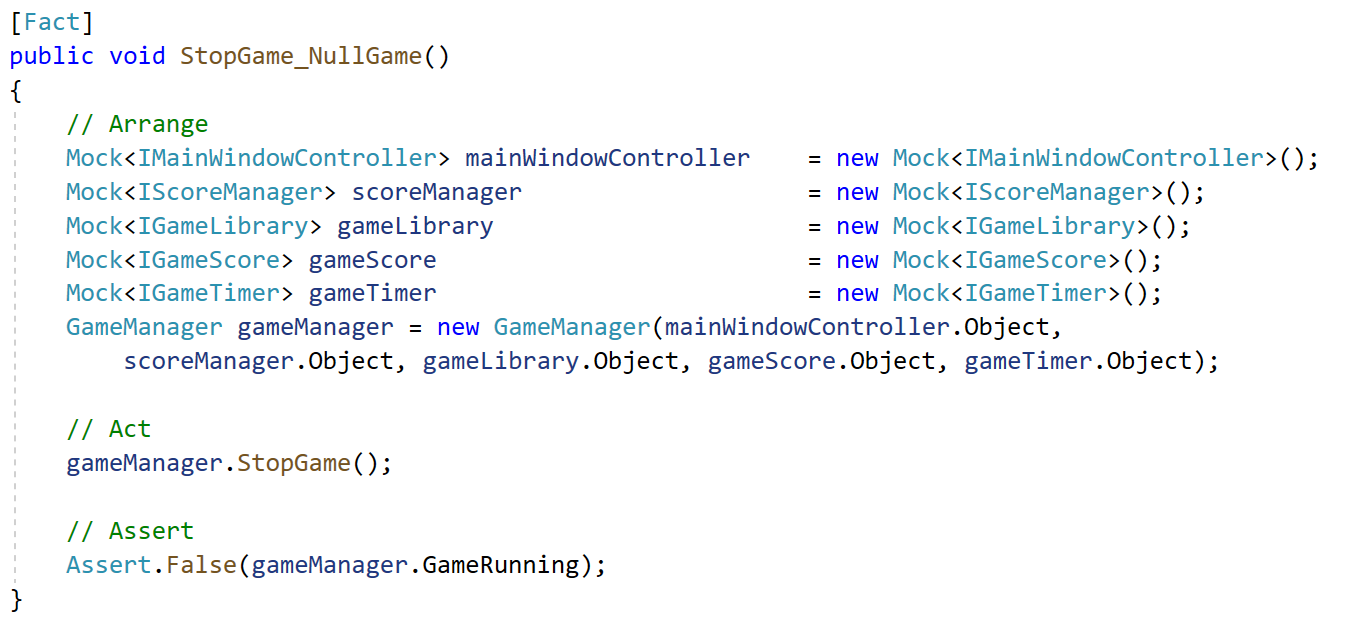
\includegraphics[width=0.95\textwidth]{Bilder/UnitTest.PNG}
\caption{\label{Abb:UnitTest}Beispiel Tests mit Mocks in AAA-Normalform}
\end{figure}

\newpage
\paragraph{Code-Coverage} Zur Bestimmung der Test Abdeckung wurde die diesbezügliche Funktionalität in Visual Studio Enterprise verwendet, welche aufgrund der Studenten Lizenz zur Verfügung steht. Die Testabdeckung des Anwendung beträgt ca. 50\% Line Coverage. Im nachfolgenden Ergebnisausschnitt dürfen dabei nur die Prozentangaben in der blau markierte Zeile beachtet werden, da dies das Projekt mit dem Anwendungscode ist.

\begin{figure}[!htb]
\centering
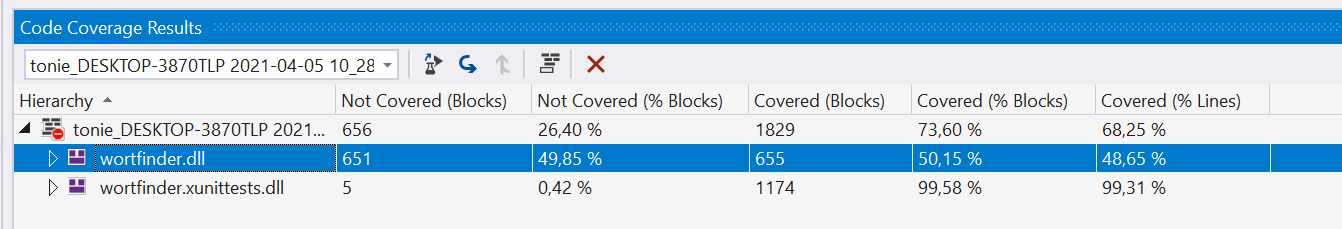
\includegraphics[width=0.95\textwidth]{Bilder/Testabdeckung.PNG}
\caption{\label{Abb:Testabdeckung}Die Ausgabe der Testabdeckung von Visual Studio}
\end{figure}

Die Abdeckung ist nicht höher, da ein Großteil der Codezeilen in den \textit{xaml} Dateien der GUI sind, welche nicht abgedeckt und nicht Unit Testbar sind. Außerdem sind wie schon erwähnt primär die wichtigen Stellen im Quellcode mit Tests abgedeckt. Unwichtigere werden eher vernachlässigt. Die Abdeckung könnte somit noch erhöht werden, wäre aber mit unnötig viel Aufwand verbunden.

\endinput